
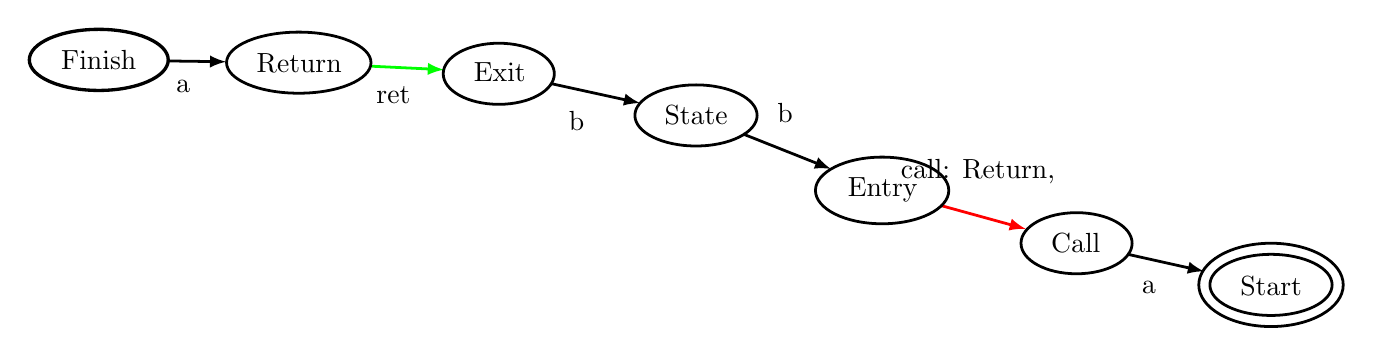
\begin{tikzpicture}[>=latex,line join=bevel,]
  \pgfsetlinewidth{1bp}
%%
\pgfsetcolor{black}
  % Edge: State -> Entry
  \draw [->] (257.98bp,70.305bp) .. controls (264.68bp,67.641bp) and (272.57bp,64.507bp)  .. (289.6bp,57.734bp);
  \definecolor{strokecol}{rgb}{0.0,0.0,0.0};
  \pgfsetstrokecolor{strokecol}
  \draw (273.03bp,77.913bp) node {b};
  % Edge: Finish -> Return
  \draw [->] (51.232bp,96.61bp) .. controls (54.564bp,96.565bp) and (58.032bp,96.518bp)  .. (71.823bp,96.332bp);
  \draw (56.37bp,87.541bp) node {a};
  % Edge: Entry -> Call
  \pgfsetcolor{red}
  \draw [->] (329.06bp,44.595bp) .. controls (335.62bp,42.79bp) and (342.97bp,40.766bp)  .. (359.7bp,36.157bp);
  \definecolor{strokecol}{rgb}{0.0,0.0,0.0};
  \pgfsetstrokecolor{strokecol}
  \draw (342.49bp,56.723bp) node {call: Return, };
  % Edge: Exit -> State
  \draw [->] (188.94bp,88.437bp) .. controls (195.68bp,86.961bp) and (203.49bp,85.254bp)  .. (220.85bp,81.457bp);
  \draw (197.96bp,75.027bp) node {b};
  % Edge: Return -> Exit
  \pgfsetcolor{green}
  \draw [->] (124.22bp,94.72bp) .. controls (129.31bp,94.475bp) and (134.68bp,94.216bp)  .. (150.23bp,93.467bp);
  \definecolor{strokecol}{rgb}{0.0,0.0,0.0};
  \pgfsetstrokecolor{strokecol}
  \draw (132.06bp,84.342bp) node {ret};
  % Edge: Call -> Start
  \draw [->] (396.2bp,27.071bp) .. controls (401.62bp,25.861bp) and (407.73bp,24.497bp)  .. (423.86bp,20.896bp);
  \draw (404bp,15.106bp) node {a};
  % Node: Finish
\begin{scope}
  \definecolor{strokecol}{rgb}{0.0,0.0,0.0};
  \pgfsetstrokecolor{strokecol}
  \draw [very thick] (26bp,97bp) ellipse (25bp and 11bp);
  \draw (26bp,96.951bp) node {Finish};
\end{scope}
  % Node: Return
\begin{scope}
  \definecolor{strokecol}{rgb}{0.0,0.0,0.0};
  \pgfsetstrokecolor{strokecol}
  \draw (98bp,96bp) ellipse (26bp and 11bp);
  \draw (98.143bp,95.976bp) node {Return};
\end{scope}
  % Node: Start
\begin{scope}
  \definecolor{strokecol}{rgb}{0.0,0.0,0.0};
  \pgfsetstrokecolor{strokecol}
  \draw (448bp,16bp) ellipse (22bp and 11bp);
  \draw (448bp,16bp) ellipse (26bp and 15bp);
  \draw (448.04bp,15.5bp) node {Start};
\end{scope}
  % Node: State
\begin{scope}
  \definecolor{strokecol}{rgb}{0.0,0.0,0.0};
  \pgfsetstrokecolor{strokecol}
  \draw (241bp,77bp) ellipse (22bp and 11bp);
  \draw (241.03bp,77.044bp) node {State};
\end{scope}
  % Node: Call
\begin{scope}
  \definecolor{strokecol}{rgb}{0.0,0.0,0.0};
  \pgfsetstrokecolor{strokecol}
  \draw (378bp,31bp) ellipse (20bp and 11bp);
  \draw (377.72bp,31.194bp) node {Call};
\end{scope}
  % Node: Entry
\begin{scope}
  \definecolor{strokecol}{rgb}{0.0,0.0,0.0};
  \pgfsetstrokecolor{strokecol}
  \draw (308bp,50bp) ellipse (24bp and 12bp);
  \draw (308.21bp,50.34bp) node {Entry};
\end{scope}
  % Node: Exit
\begin{scope}
  \definecolor{strokecol}{rgb}{0.0,0.0,0.0};
  \pgfsetstrokecolor{strokecol}
  \draw (170bp,92bp) ellipse (20bp and 11bp);
  \draw (170.37bp,92.497bp) node {Exit};
\end{scope}
%
\end{tikzpicture}
